\documentclass[12pt]{jreport}
\usepackage{comment}
\usepackage{./sty/eclepsf}
\usepackage{tascmac}
\usepackage{tabularx}
\usepackage{listliketab}
\usepackage[longnamesfirst]{natbib}
\usepackage[dvipdfmx]{graphics}
\usepackage[dvipdfmx]{graphicx}
\usepackage[dvipdfmx]{color}
\usepackage{subfigure}
\usepackage{alltt}
\usepackage{here}
\usepackage{afterpage}
\usepackage{./sty/ncodeline}

\usepackage{amsmath, amssymb, amsthm}
\usepackage{color}


%\usepackage[dvipdfmx, colorlinks, breaklinks,%
\usepackage[dvipdfmx, breaklinks,%
bookmarks=true, bookmarksnumbered=true,%
bookmarkstype=toc, bookmarksopen=true,bookmarksopenlevel=3,%
pdftitle={RG},%
]{hyperref}
\usepackage{bookmark}

\AtBeginDvi{\special{pdf:tounicode EUC-UCS2}}

\usepackage{fancyhdr}

\usepackage{./sty/algorithm}
\usepackage{./sty/algorithmic}

\usepackage{indentfirst}
\usepackage{url}
\usepackage{listings,./sty/jlisting}



%% Add Mathematical Notation Shortcuts and Macros here:
\def\ball{\mathbb{B}}
\def\reals{\mathbb{R}}
\def\LPAV{{\sf LPAV}}
\def\PAV{{\sf PAV}}
\def\GLMt{\textsf{GLM-tron}}
\def\KAF{\textsf{K-AF-tron}}
\def\Liso{\textsf{L-Isotron}}
\def\Iso{\textsf{Isotron}}
\def\err{\mathrm{err}}
\def\E{\mathbb{E}}
\def\herr{\widehat{\mathrm{err}}}
\def\eps{\varepsilon}
\def\heps{\hat{\varepsilon}}

%% Shortcuts
\def\fraconem{\frac{1}{m}}
\def\hatyti{\hat{y}^t_i}
\def\sumionetom{\sum_{i=1}^m}
\def\realstozo{\reals \rightarrow [0, 1]}
\def\baryi{\bar{y}_i}
\def\tildeyti{\tilde{y}^t_i}

%% Additional definitions (Ohad)
\newtheorem{proposition}{Proposition}
\newcommand{\norm}[1]{\left\|#1\right\|}
\newcommand{\inner}[1]{\langle#1\rangle}
\newcommand{\Ucal}{\mathcal{U}}
\newcommand{\Wcal}{\mathcal{W}}
\newcommand{\Fcal}{\mathcal{F}}
\newcommand{\Ncal}{\mathcal{N}}
\newcommand{\lemref}[1]{Lemma~\ref{#1}}
\newcommand{\thmref}[1]{Thm.~\ref{#1}}

\newcommand{\lnorm}[1]{\ensuremath \left\| #1 \right\|}

%% Theorems
\newtheorem{lemma}{Lemma}
\newtheorem{thm}{Theorem}




\def\lstlistingname{プログラム}

\lstset{%
 language={C++},
 %backgroundcolor={\color[gray]{.85}},%
 basicstyle={\small\ttfamily},%
 identifierstyle={\small},%
 commentstyle={\small\itshape},%
 keywordstyle={\small\bfseries},%
 ndkeywordstyle={\small\ttfamily},%
 stringstyle={\small\ttfamily},
 frame={tb},
 framesep=1zw,
 breaklines=true,
 numbers=left,%
 xrightmargin=0zw,%
 xleftmargin=1.5zw,%
 numberstyle={\scriptsize},%
 stepnumber=1,
 numbersep=1zw,%
 lineskip=-0.5ex%
}

\usepackage{amssymb}
%\usepackage{supertabular,multirow}

\usepackage{array}
\newcolumntype{M}[1]{>{\centering\arraybackslash}m{#1}}

% A4  size: 297mm*210mm %1pt = 0.35mm
\setlength{\topmargin}{-3.4mm} % 10pt 25.4mm - 3.4mm = 22mm
\setlength{\oddsidemargin}{-0.4mm} % 25.4mm - 0.4mm = 25mm
\setlength{\evensidemargin}{-0.4mm} % 25.4mm - 0.4mm = 25mm
\setlength{\textheight}{231mm} % 660pt % original is 225.75mm 645pt
\setlength{\textwidth}{160mm} % 457pt

\renewcommand{\topfraction}{.99}
\renewcommand{\textfraction}{.0}
\renewcommand{\floatpagefraction}{.99}
\renewcommand{\bibname}{参考文献}


\pagestyle{fancy}
\lhead[]{}

\makeatletter
\def\chaptermark#1{\markboth {\ifnum \c@secnumdepth>\m@ne
\@chapapp\ \thechapter \@chappos\ \fi #1}{}}
\makeatother

% タイトル
\def\title{カーネル関数を用いた汎用的な活性化関数の開発}
% 英語タイトル
\def\etitle{\LaTeX Template for RG 2020}
% 著者(日本語)
\def\author{神保和行}
% 著者(英語)
\def\eauthor{Kazuyuki Jimbo}
% 学部・研究科
\def\dept{慶應義塾大学大学院 環境情報学部}
% 学部・研究科(英語)
\def\edept{Keio University Faculty of Environment and Information Studies}

\begin{document}

\pagenumbering{roman}
\begin{titlepage}
  \begin{center}
    \begin{large}
      卒業論文   2020年度(令和02年)\\
      \vspace{24pt}
      \title
      \end{large}
  \end{center}
  \vspace{40em}
  \begin{flushright}
    \large \dept\\
    \author
  \end{flushright}
\end{titlepage}

\thispagestyle{empty}


卒業論文要旨 - 2020年度 (令和02年度)
\begin{center}
\begin{large}
\begin{tabular}{|M{0.97\linewidth}|}
    \hline
      \title \\
    \hline
\end{tabular}
\end{large}
\end{center}

~ \\



近年機械学習では、ニューラルネットワークにおける活性化関数として、シグモイド関数やReLU関数などの一般的に用いられてきた。
ニューラルネットワークにおける活性化関数は、その種類や問題に応じて最適な活性化関数を経験則に基づいて調整していた。
一方,統計学の分野では,リンク関数が未知の場合には,カーネル関数を用いてノンパラメトリックに推定するという手法が推定されている。
そこで本論文は事前に関数の形を指定しないカーネル関数を用いた活性化関数を提案する。
さらに、実際のデータセットを用いて、ニューラルネットワークの出力層を本論文で提案する方法に置き換えることにより
従来の活性化関数と同等かそれ以上の精度で予測できること示した。


~ \\
キーワード:\\
\underline{1. ディープラーニング},
\underline{2. 活性化関数},
\underline{3. ノンパラメトリック},
\underline{4. カーネル関数}
\begin{flushright}
\dept \\
\author
\end{flushright}

\thispagestyle{plain}
\clearpage

Abstract of Bachelor's Thesis - Academic Year 2020
\begin{center}
\begin{large}
\begin{tabular}{|p{0.97\linewidth}|}
    \hline
      \etitle \\
    \hline
\end{tabular}
\end{large}
\end{center}

~ \\


In recent years, in machine learning, sigmoid functions and ReLU functions have been commonly used as activation functions in neural networks.
The optimal activation function was adjusted empirically according to the type of activation function and the problem.
On the other hand, in the field of statistics, when the link function is unknown, the method of nonparametric estimation using kernel functions has been estimated.
Therefore, this paper proposes an activation function using a kernel function that does not assume the form of the function in advance.
Furthermore, by replacing the output layer of the neural network with the method proposed in this paper using a real data set, it is shown that the prediction accuracy is as good as or better than the conventional activation function.


~ \\
Keywords : \\
\underline{1. Deep lerning},
\underline{2. Activation Function},
\underline{3. Non parametric},
\underline{4. Kernel Function}
\begin{flushright}
\edept \\
\eauthor
\end{flushright}

\thispagestyle{plain}
\clearpage

\tableofcontents\thispagestyle{plain} %目次
\clearpage
\listoffigures\thispagestyle{plain} %図目次
\clearpage
\listoftables\thispagestyle{plain} %表目次
\clearpage

\pagenumbering{arabic}
\chapter{序論}
\label{introduction}

本章ではまず, 本研究を取り巻く社会の背景について述べる. そして本研究の解決する
課題及び課題を解決する意義, 解決するための手法を提示する. 最後に本論文の構成を外
観し, 序論を締める.

\section{はじめに}
\label{introduction:background}

\subsubsection{背景}


近年、画像認識や音声認識といった分野で機械学習の中でもディープラーニングと呼ばれる分野が急速発展し、自動運転やスマートスピーカーといったプロダクトとして人々の日常の中にも応用され始めている。
機械学習はプログラミングを容易にするPytorch~\cite{pytorch}やTensorflow~\cite{tensorflow}と呼ばれるライブラリの開発も積極的に行われているだけではなく
ソニーのNeural Network Console~\cite{sony}を筆頭とした、非エンジニアにも使いやすいGUIベースのツールも多数開発され続けている。
これらは機械学習におけるニューラルネットワークの構築を容易にするだけではなく、学習アルゴリズム自体も抽象化され複雑な数式を理解せずとも使用できるようになっている。
また、ニューラルネットワークを構築する重要な要素の一つに活性化関数がある。
この活性化関数には、SigmoidやReLU~\cite{ReLU}などの一般的に用いられてきた。
そしてこれらは問題やデータに応じて最適な活性化関数を経験則に基づいて調整していた。
また、ニューラルネットワークでは特に出力層のアウトプットを考慮した活性化関数の組み合わせを採択することが多く、例えばResnet50~\cite{resnet50}では、
問題が分類ということを考慮され、中間層は全てReLU、出力層はSigmoidなどといった組み合わせが使用されている。

一方,統計学の分野では,リンク関数が未知の場合には,ノンパラメトリックな手法に基づきモデルを推論する幾つかの手法が考案されている。
カーネル密度推定を用いてノンパラメトリックに推定するという手法がIchimura(1993)~\cite{ichimura}によって提案されている。

\subsubsection{課題・手法}

ニューラルネットワーク構築の際の課題として、問題に応じた最適な活性化関数が未だわかっていないことが挙げられる。
全ての課題に同一の活性化関数を流用するのではなく、各課題においてその都度適切な活性化関数を導くことができればより良い精度が出せることが予想される。
特に出力層に用いる活性化関数はデータセットや問題の種類を意識する必要があり、精度に非常に直結するだけでなく、初学者にとっての構築を難しくする
そこで本論文は事前に関数の形を指定しないカーネル密度推定を用いた活性化関数を提案する。
本間研究ではカーネル密度推定とトレーニングデータの少数の点を用いて活性化関数の推論をするアルゴリズムを構築する。
提唱されたIchimura(1993)の方法では、トレーニングデータの全てを活性化関数の計算に使用する必要があったが、
ディープラーニング等のデータ量が非常に大きい場合での応用を考え計算時間を現実的なものにするため、使用するデータ点を可変にすることが可能なアルゴリズムを提案した。

本論文では以下の課題を解決した。
\begin{itemize}
  \item 出力層に用いる活性化関数を状況に応じた適切な形に変わる汎用的な関数を導き、高い精度を出せるようにした。
  \item そのような関数を用いることで、データセットの形等の専門的な知識を理解しなくて済むようになり、ニューラルネットの構築を容易にした。
\end{itemize}

\subsubsection{貢献}

今後本研究で提案するカーネル密度推定を用いた活性化関数をK-AFと表記する。
K-AFは実際のデータセットを用いて、ニューラルネットワークの出力層を本論文で提案する方法に置き換えることにより従来の活性化関数と同等かそれ以上の精度で予測できること示した。
本研究における主な貢献を以下にまとめる.

\begin{itemize}
  \item カーネル密度推定を用いた汎用的な活性化関数で実用的なものを完成させた。
  \item K-AFはさまざまなデータセットにおいて既存の活性化関数によりより良い精度を出すことを達成した。
  \item K-AFはいくつかのデータセットでは高い学習率でも安定した学習精度を出すことに成功した。
  \item K-AFを用いることによりデータセットに応じて出力層の活性化関数の形は従来のものではないことを示した。
  \item K-AFが勾配消失しないための条件を探求した。
\end{itemize}


\section{本論文の構成}

本論文における以降の構成は次の通りである.

~\ref{background}章では,ノンパラメトリックモデル、カーネル密度推定などといった本研究へとつながる背景の解説し、これらの手法における課題を洗い出す。
~\ref{proposed}章では,本研究におけるカーネル密度推定を用いた活性化関数についての解説を行い、提案手法の解説の詳細を述べる。
~\ref{implementation}章では,~\ref{proposed}章で述べた手法の実装及び、実装における留意点を述べる。
~\ref{evaluation}章では,\ref{background}章で求められた課題に対しての評価を行い,考察する.
~\ref{conclusion}章では、実験の結果に対する考察を行い,本研究を行う上で浮上した提案手法の限界を示し,今後の研究方針についてまとめる






%%% Local Variables:
%%% mode: japanese-latex
%%% TeX-master: "../thesis"
%%% End:

\chapter{背景}
\label{background}

本章では本研究の背景について述べる.
まず機械学習における活性化関数のの役割について明確にする。
また、統計学において活性化関数に相当する概念がどのように応用されてきたか述べる。
活性化関数について概説し、現在の機械学習における活性化関数の抱える問題点を明らかにする。
次に、活性化関数の他に、ニューラルネットワークにおける精度を向上させるいくつかの構成要素について述べる。
本研究の問題点の解決に必要な、ノンパラメトリックモデルとその具体例であるカーネル密度推定を導入する。
最後に、実社会において機械学習を行う上での問題点や課題を述べ、本研究が取り組むべき課題を明確にする。



\section{活性化関数}

\begin{figure}[hbtp]
    \begin{center}
        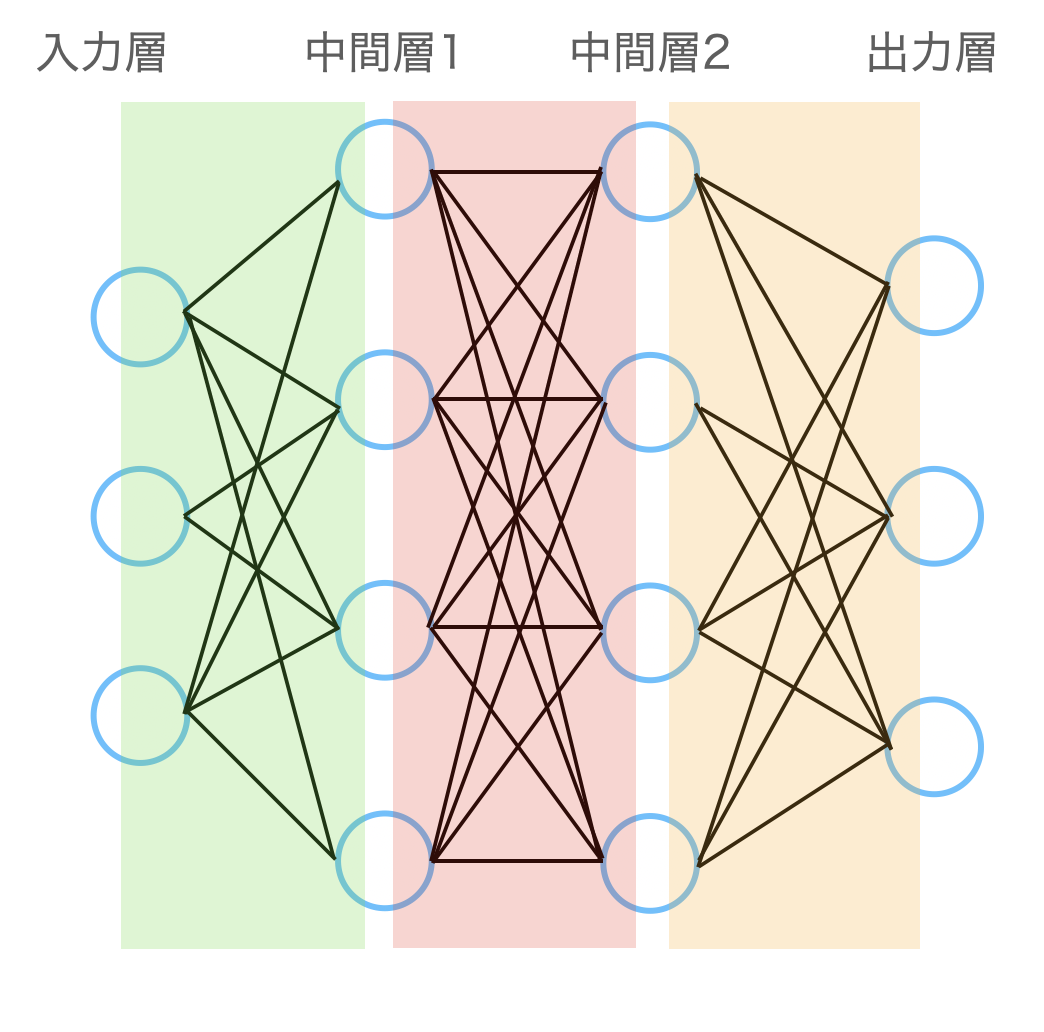
\includegraphics[width=10cm]{asset/neural_network1.png}
            \caption{活性化関数の領域。緑、赤、オレンジの領域によって使われる活性化関数が変わることが多い。}
            \label{neural_network1}
    \end{center}
\end{figure}

また、概要を述べるにあたってニューラルネットワークの用語を定義する。活性化関数は
図の黄色で囲った活性化関数を出力層の活性化関数、赤色部分を中間層の活性化関数、緑色部分を入力そうの活性化関数と呼ぶことにする。

ディープラーニングの活性化関数に関する最近の研究はまだ多く、様々な実験が 行われている~\cite{study_af}。
活性化関数の歴史はシグモイドという統計学的にも馴染み深いロジスティック回帰のモデルから始まった。
ニューラルネットワークの層に活性化関数を適用する過程を以下に示す。
$ w_i$ を重み、$ \mathbf{X}_i $ は入力の値、$ b $はバイアス、$z$ は出力、$ g $ を活性化関数とした時
$ z=g(y)=g(\sum w_i \mathbf{X}_i+b) $ 
このように用いられる。
その後TanhやXavierのReLU(2011)~\cite{ReLU}などといったより計算に適した活性化関数が発見されてきた。
特にReLUに関しては現在のディープラーニングなどの深層ニューラルネットワークにおいても未だ応用されており、実用的にもその有用性が示されていることがわかる。

長年にわたり、性能を向上させ、ReLUの欠点に対処する多くの活性化関数が提案されてきたが、その中にはLeaky ReLU ~\cite{leaky_relu}、ELU~\cite{elu}、SELU~\cite{selu}などが含まれる。
Prajit RamachandranのSwish(2017)~\cite{swish}は、$ f(x)=x {\bf sigmoid}(\beta x) $ と定義できるが、よりロバストな活性化関数であることが証明され、ReLUと比較して結果が大幅に改善された。
活性化関数はそれまで単調増加な関数が使われることが多かったが、Swishで単調増加である必要なく、汎用的に精度が向上することがわかった。
またそのような活性化関数の例としてDiganta. MisraのMish(2019)~\cite{Mish}と言うものもあげらている。

\begin{table}[htbp]
    \begin{center}
        \caption{活性化関数の種類}
        \vspace{2mm} 
        \label{|class_af|}
        \begin{tabular}{cp{5cm}cc}
        活性化関数の数式              & 数式 \\
        \hline
        Sigmoid            & $ \cfrac{1}{1 + \mathrm{exp}(x)} $ \\
        \hline
        Tanh               & tanh(x) \\
        \hline
        \multirow{5}{*}{ReLU}        &  \[{\rm output} =
            \begin{cases} 
            0 &\text{when $ x < 0 $ }\\
            x &\text{when $ x \geq 0 $ else} \\
            \end{cases}
            \] & & \\
        \hline
        Swish           & $ x\cdot {\rm sigmoid}(\beta x) $ \\
        \hline
        Mish           & $ x\cdot {\rm tanh}(\log (1 + \mathrm{exp}(x) )) $ \\
        \hline

        \end{tabular}
    \end{center}
\end{table}


\subsection{勾配爆発問題}
勾配爆発問題とは、ニューラルネットワークの設計において、勾配が発散することで学習が進まなくなる技術的な問題のことである。
勾配発散の問題はRNN~\cite{rnn}などの行列の積が絡む問題やGAN~\cite{gan}などの誤差関数が不連続のな場合では簡単に発生する問題である。
これを対処するためには簡単な手法としてパラメータの勾配の上限値を決めるクリッピングという操作を用いる方法などが挙げられる。
勾配を$ g $、勾配の上限値を$ M $で表現した場合に、勾配を以下式(\ref{eq:hassan})のように変換する。


\begin{eqnarray}
\dot g = \frac{M}{\|g\|} g
\label{eq:hassan}
\end{eqnarray}




\section{統計学における位置付け}

\begin{figure}[hbtp]
        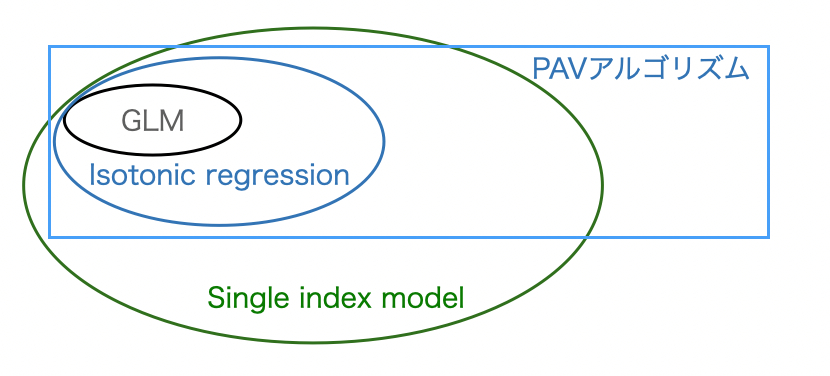
\includegraphics[width=15cm]{asset/machine_statistics.png}
            \caption{機械学習と統計学の繋がり}
            \label{glm}
\end{figure}

活性化関数の概念は統計学におけるリンク関数と呼ばれるモデルの汎用性を高める動きに始まり、機械学習へと応用されている。
本項目ではその理解に必要な知識を述べていく。



\subsection{一般化線形モデルとは}


\begin{figure}[hbtp]
        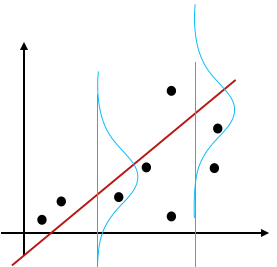
\includegraphics[width=6cm]{asset/glm1.png}~~~~~ ~~~~~ 
        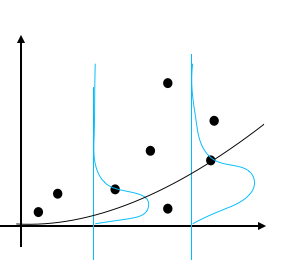
\includegraphics[width=6cm]{asset/glm2.png}
            \caption{一般化線形モデルの必要性}
            \label{glm}
\end{figure}

説明変数を$ X $, パラメータを$ W $で表現し、従属変数を$ Y $、誤差を$ \epsilon \sim \mathcal{G}(0, \sigma^2) $で表現すると、一般線形モデルは以下の式で表現することができる。

\begin{eqnarray}
\mathbf{Y} = \mathbf{X} \cdot  \mathbf{W} + \epsilon
\label{eq:senkei}
\end{eqnarray}
またこれは$ \mathbf{Y} $の期待値を使って表現すると上記は
\begin{eqnarray}
    \mathrm{E}[\mathbf{Y}] &=& \mathrm{E}[\mathbf{X} \cdot  \mathbf{W} + \epsilon] \\
    \mathrm{E}[\mathbf{Y}] &=& \mathrm{E}[\mathbf{X} \cdot  \mathbf{W}] + \mathrm{E}[\epsilon] \\
    \mathrm{E}[\mathbf{Y}] &=& \mathbf{X} \cdot  \mathbf{W}
\label{eq:link}
\end{eqnarray}
である。
しかしながら、上記の式の展開では$ \epsilon $が正規分布に従うことを想定した、すなわち従属変数$ Y $がガウス分布に従うことを仮定したが、実際は図\ref{glm} のように、誤差の分布にガウス分布を仮定すると、正確さが失われることがある。
そこで、従属変数をある関数 $ G $ で変換してからモデル化することでモデルの正確さが向上する。
すなわち、$ \mathrm{E}[\mathbf{Y|X}] = \mathbf{X} \cdot  \mathbf{W} $ に対して$ G(\mathrm{E}[Y|X]) = \mathbf{X} \cdot  \mathbf{W} $ となるような$ G $ を取り入流。
またこの$ G $ の逆関数 $ G^{-1} $をリンク関数と呼ぶ。
一般線形モデルに対して、リンク関数を加えた式を以下に記す。
\begin{eqnarray}
E[\mathbf{Y|X}]=G^{-1} (\mathbf{X}\cdot  \mathbf{W})
\label{eq:link}
\end{eqnarray}

一般に誤差構造が決まれば、リンク関数も自動的に決まる。
ガウス分布の場合のリンク関数は$ G(U) = U $である。
これらの結果は$ G^{-1} $を単調増加な任意の関数に置き換えることでさまざまなモデルを表現することが可能になる。


\subsection{シグモイド関数とロジスティック回帰}
\begin{eqnarray}
G(\mathbf{Y})=\mathbf{X}\cdot  \mathbf{W}
\end{eqnarray}
とした時、
\begin{eqnarray}
G=\log \bigl(\frac{y}{1-y}\bigr)
\end{eqnarray}
とする。一般的にこれはロジット関数と呼ばれる。
これを左辺が$ y $になるように変形すると,

\begin{eqnarray}
\log \bigl(\frac{y}{1-y}\bigr) = z \\
y = \frac{1}{1 + \exp(-z)}
\end{eqnarray}
右辺を$ z $を関数にすると

\begin{eqnarray}
g(z) = \frac{1}{1 + \exp(-z)}
\end{eqnarray}
となり、これはシグモイド関数である。
$ g(z) $はロジスティック関数でもあり、


\begin{eqnarray}
y = \frac{1}{1 + \exp (\mathbf{X} \cdot  \mathbf{W})}
\end{eqnarray}
より、ロジスティック回帰であることも示される。 \\

これらにより、ニューラルネットワークに出てくるシグモイど関数が潜在的に統計学の世界でも出てくることがわかる。






\begin{figure}[hbtp]
    \begin{center}
        \begin{tabular}{c}
            \begin{minipage}{0.40\hsize}
                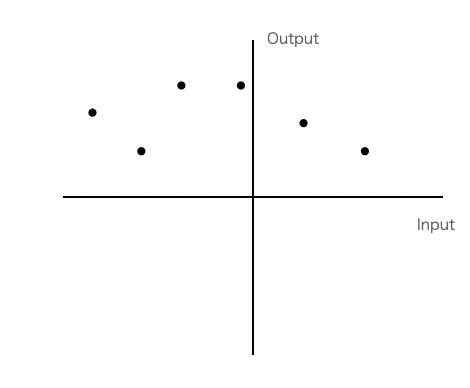
\includegraphics[clip, width=5cm]{asset/k_af_band1.png}
                    \caption{データ点がまばらに存在する。}
                    \label{k_af_band1}
            \end{minipage}
            \hspace{10pt}
            \begin{minipage}{0.40\hsize}
                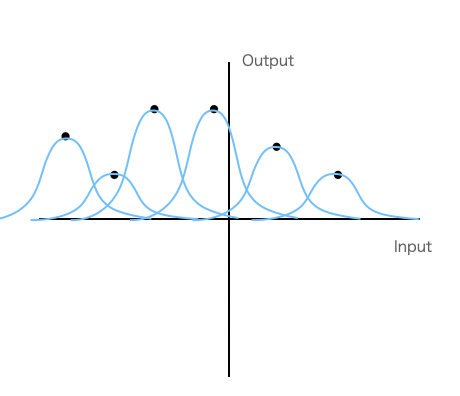
\includegraphics[clip, width=5cm]{asset/k_af_band2.png}
                    \caption{カーネル関数、今回はガウス関数でその周辺ごと近似する。}
                    \label{k_af_band2}
            \end{minipage}
            \hspace{10pt} \\
            \vspace{10pt} \\
            \begin{minipage}{0.40\hsize}
                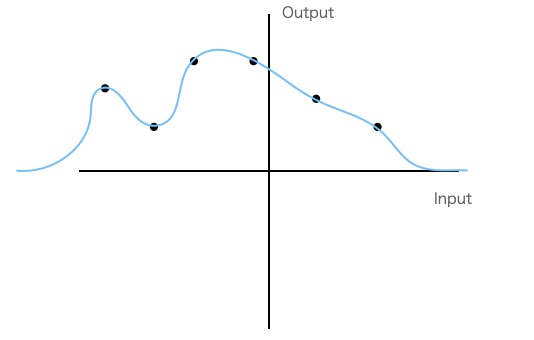
\includegraphics[clip, width=5cm]{asset/k_af_band3.png}
                    \caption{点の周辺のカーネル関数を足し合わせた時にできる関数}
                    \label{k_af_band3}
            \end{minipage}
        \end{tabular}
    \end{center}
\end{figure}


\subsection{ノンパラメトリックとカーネル密度推定}
統計学において、パラメータで表現されるモデルや確率分布を使用すものをパラメトリックな手法として分類するが、パラメータを使用せずモデルを表現する手法をノンパラメトリック手法という。
ノンパラメトリックを代表する手法の一つにカーネル密度推定と呼ばれる手法がある~\cite{kernel_density}。
これは、ある母集団のデータが与えられたとき、カーネル関数を用いてその関数を推定する手法である。
カーネル関数とは、与えられた領域内で積分した時に1となり、対称性を持つものとしてイメージして良い。
カーネル関数の代表例としてガウス関数があげられる。

$ K $をカーネル関数 $ u \in R $ とした時、カーネル関数の定義は以下である。

\begin{itemize}
  \item $ \int^{+ \infty}_{- \infty} K(u)du = 1 $
  \item $ K(-u) = K(u) $
\end{itemize}


この時、カーネル密度推定法とは、$ \mathbf{X}_n $をデータ、推定すべき関数を$ f $ カーネル関数を $ K $ バンド幅を $ h $ としたとき、以下の式で表現することができる。


\begin{eqnarray}
f(x) = \frac{1}{nh} \sum^n_{i=1}K \bigl( \frac{x - \mathbf{X}_i}{h}\bigr)
\label{eq:k-af}
\end{eqnarray}
\ref{k_af_band1}のようにまばらに存在するデータ点の周辺に、\ref{k_af_band2}のようにカーネル関数をおき、任意のバンド幅で足し合わせ近似していくようなものである。






\subsection{セミパラメトリックモデルとシングルインデックスモデル}

統計学の世界では、セミパラメトリックモデルというノンパラメトリックな手法とセミパラメトリックな手法を組み合わせた手法が存在する。
その中の一つの代表的な手法の中にシングルインデックスモデルと呼ばれる手法が存在する。
シングルインデックスモデル(SIM)とは、未知の関数 $ g $、従属変数 $ Y $、説明変数$ X $、パラメータ$ W $、誤差項 $ \epsilon $と置いた時、以下のように表される式である。

\begin{eqnarray}
Y = g(\mathbf{X} \cdot  \mathbf{W}) + \epsilon
\label{eq:k-af}
\end{eqnarray}

SIMは未知の関数$ g $を推定しながらパラメータ $ W $を求めていく問題に帰着されるため、ノンパラメトリックとパラメトリックが混ざった手法であるセミパラメトリックモデルとして表現される理由である。
この$ g $は、一般化線形モデルのリンク関数$ G^{-1} $ をさらに一般化した単調増加性を無くしたモデルだと考えることができる。
SIMの有名なモデルの一つにisotonic regressionと呼ばれるものがある。

\begin{figure}[hbtp]

    \begin{center}
        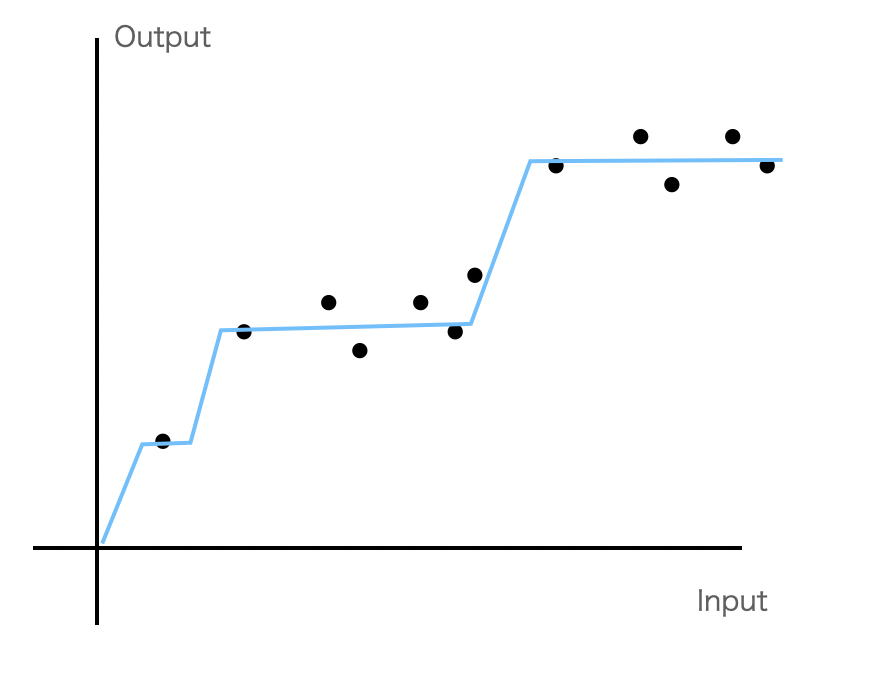
\includegraphics[width=10cm]{asset/isotonic_regression.png}
            \caption{シングルインデックスモデルの例の一つのisotonic regression}
            \label{isotonic_regression}
    \end{center}
\end{figure}

isotonic regressionは単調増加性等の制約を仮定したSIMの一つで、化学分野や経済分野に応用されている。


\subsection {セミパラメトリックモデルと機械学習学習}

セミパラメトリックにモデルを推定する手法は統計学ではIchimura(1993)~\cite{ichimura}から始まり、PAVアルゴリズムとしてAdam Tauman Kalai(2008)~\cite{isotron}によりその有用性が確かめられた。

\subsubsection{Ichimuraの手法}

SIMの未知の関数をleave one out法を用いたカーネル密度推定法と最尤推定により導く試みはIchimura(1993)~\cite{ichimura}や Klein(1993)~\cite{klein}によって提案され始めた。

Ichimura(1993)の手法はSingleIndexModelのノンパラメトリック関数を以下の式で近似する手法である。


\begin{eqnarray}
G(\mathbf{X}_iw)=\frac{\sum_{i\neq j} K\left(\frac{\mathbf{X}_j w - \mathbf{X}_i w}{h}\right)\mathbf{Y}_j}{\sum_{i\neq j} K\left(\frac{\mathbf{X}_j w - \mathbf{X}_i w}{h}\right)}
\label{eq:ichimura}
\end{eqnarray}

ここで、$ K $はカーネル関数である。$ i \neq j $ とすることにより、$ \mathbf{X}_i $を入力した時の値が$ y_i $へと過剰適合しないようにするためである。



\subsubsection{PAVアルゴリズム}

SIMやisotonic regressionを機械学習に応用する試みはAdam Tauman Kalai~\cite{isotron}のPAVアルゴリズムと呼ばれる手法で、分類問題の応用へと繋がった。
isotonic regression自体は回帰問題として発明された手法であったが、これによりアルゴリズム的に分類問題がセミパラメトリックな手法を用いて解くことが可能であることが発見された。
この手法をベースにSham Kakade(2011)~\cite{efficient_sim}やRavi Ganti(2015)~\cite{lsim}などによってより高速で汎用的なisotonic regressionを応用したセミパラメトリックモデルの分類問題の解法のアルゴリズムが導かれた。


\section{勾配法と学習における知識}
機械学習の問題の多くは学習の際の最適なパラメータを探索する。最適なパラメータとは損失関数が最小値を撮る時の値のことである。
勾配法とは関数の勾配方向に閾値を移動させることで、関数の最小値を見つける方法のことである。特にニューラルネットにおいては最小値を見つけるために、勾配法がよく用いられる。
損失関数を$ E $, $ w_i $をiステップ目のパラメータとした時、勾配法を数式で表すと以下のようになる。

\begin{eqnarray}
w_{i + 1} = w_i - \mu \frac{\partial E}{\partial w}
\label{eq:learning_rate}
\end{eqnarray}

複雑な損失関数を最小化させるためのテクニカルな手法として、学習率、初期パラメータ、正則化などと言ったものが挙げられる。
本項ではこれらについて必要な概念を述べる。
\subsection{LearningRate(学習率)}

LearningRateとはハイパーパラメータの一つで、式(\ref{eq:learning_rate})の$ \mu $にそうとする部分でらう。
LearningRateは大きいほど収束の可能性は小さくなり、小さいほど学習が遅くなる。
活性化関数の性能評価の一つに、大きな学習率に対しての収束性能のがあげられる。


\subsection{Initializer(重みの初期化)}
ニューラルネットワークの学習効率は、重みの初期値によって大きく変わることが知られている。
例えば初期値を全て$ 0 $に固定すると、逆誤差伝播の影響で重みが均一になることにより、重みを多く持つ意味がなくなる。
この問題を解消するために、学習のテクニックとして以下のような手法がある。
また、重みの初期化手法を総称してInitializerと呼ぶ。

\subsubsection{Xavier initializer}
Xavier(2010)~\cite{xavier}によって提唱された重みの初期化手法の一つで、現在最もニューラルネットワークの学習で利用されてる手法である。
ニューラルネットワークの$ i $層の重みの数を$ n_{i} $、重みを$ w_i $、一様分布を$U$ で表現した時

\begin{eqnarray}
w_{i} \sim U \bigl[ - \frac{\sqrt{6}}{ \sqrt{n_i + n_{i+1}} }, \frac{\sqrt{6}}{ \sqrt{n_i + n_{i+1} }} \bigr]
\end{eqnarray}
で初期化する手法である。これにより初期化すると、重みの分布が広がりを持つことが知られている。
活性化関数がLinear、Sigmoid、Tanhの時に有効に働く。

\subsubsection{KaimingUniform}
Kaiming He(2015)~\cite{kaiming}によって提案された初期化の手法で、以下の分布から重みをサンプリングする。

\begin{eqnarray}
w_{i} \sim U \bigl[ - \frac{\sqrt{6}}{ \sqrt{n_{i+1}} }, \frac{\sqrt{6}}{ \sqrt{ n_{i+1} }} \bigr]
\end{eqnarray}

主にReLUに有効になる。


\subsection{Regularizer(正則化)}
ニューラルネットワークは訓練データを過剰に学習すると未知データへの予測精度が落ちることがある。
これはモデルが訓練データに対して過剰に学習したため、はずれ値やノイズまで学習してしまうことが問題であると考えることができる。
このような現象を過学習というが、この過学習を防ぐためにパラメータに対して一種の罰則をかけるようなことが一般的に行われている。

損失関数を$ E(w) $とした時に、最適化する関数を$E(w)$の代わりに以下の式を用いる。

\begin{eqnarray}
E(w) + \lambda \frac{1}{p}\|w\|^p_p
\label{eq:regu}
\end{eqnarray}


ここで$ w $はパラメータベクトルで$ \| \cdot \| $はL1ノルム(p=1)やL2ノルム(p=2)などである。$ \lambda $ はハイパーパラメータである。


\begin{figure}[hbtp]
    \begin{center}
        \begin{tabular}{c}
            \begin{minipage}{0.40\hsize}
                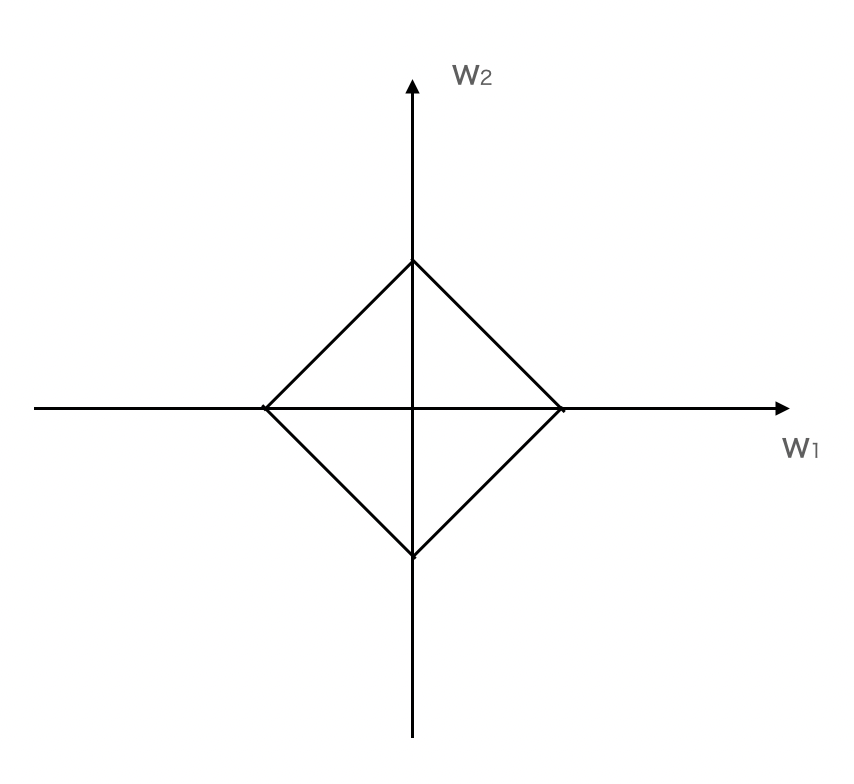
\includegraphics[clip, width=5cm]{asset/l1norm.png}
                    \caption{パラメータが二つの時のL2ノルムのイメージ図。パラメータが二つある時、その合計値($ \sum_i w_i $)が$ 1 $の点を取ると、一つのパラメータを$ 0 $にすることが最も大きくなる。}
                    \label{l1norm}
            \end{minipage}
            \hspace{10pt}
            \begin{minipage}{0.40\hsize}
                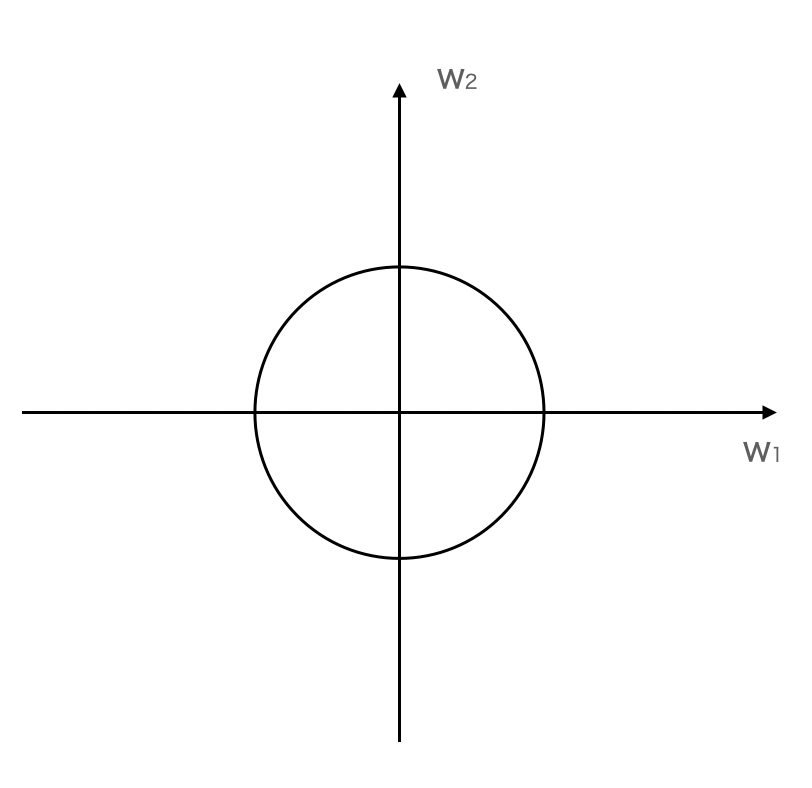
\includegraphics[clip, width=5cm]{asset/l2norm.png}
                    \caption{パラメータが二つの時のL2ノルムのイメージ図。パラメータの合計値その合計値($ \sum_i w_i $)が$ 1 $の時は$ w_1 = w_2 = 0.5 $の時が最も値が小さくなるので、より高次元で考えるとこの値を大きくするのは均一的な重み分布であることが望ましい。}
                    \label{l2norm}
            \end{minipage}
        \end{tabular}
    \end{center}
\end{figure}




\subsubsection{L1ノルム}
L1正則化は余分なパラメータ(説明変数)を省くことを目的とした手法である。
\ref{eq:regu}の式を考えると、モデルに必要ないパラメータを$ 0 $にすることが損失関数の最小化につながることがわかる。
この結果は、主に次元の圧縮などに対して応用することも可能である。

\subsubsection{L2ノルム}
L2ノルムの値を$ L2 $、L1ノルムの値を$ L1 $、またパラメータの合計値($ \sum_i w_i $)が等しい場合においては

\begin{eqnarray}
L2 < L1
\label{eq:norm uneq}
\end{eqnarray}
であることがわかる。これはL1ノルム同様に一つのパラメータを$ 0 $に対することの影響度が関数全体に対して小さいことを表していると考えられる。
以上によりL2ノルムの最小化は、均一的にパラメータを小さくすることで、最小化を図ることができる。
以上によりL2ノルムの罰則を足した合わせた損失関数により最小化したニューラルネットワークはパラメータ数が多いため、"表現力に優れている"と表現することが可能である。
これは過学習の回避に用いることができる。


\subsection{データセットの選択}
ニューラルネットワークの最適化の際に学習データセットをどのように用いるかによって性能が大きく変わることが知られている。
データセットの集合を$ D $ 大きく分けて以下の三つの方法があることが知られている。

\begin{table}[htbp]
    \begin{center}
        \caption{実験に用いるデータ集合の表現方法}
        \vspace{2mm} 
        \begin{tabular}{l*{2}{c}r}
        扱うデータ      & 名称 & 説明 \\
        \hline
        $ \mathcal{D}_i \subseteq \mathcal{D} $          & ミニバッチ学習  & データを部分的にランダムで取り出して学習を行う \\
        $ d_i \in \mathcal{D} $                & オンライン学習 & データを一つ取り出して学習を行う  \\
        $ \mathcal{D}  $      & バッチ学習 & 全てのデータを用いて学習する \\
        \end{tabular}
    \end{center}
\end{table}

バッチ学習は安定した学習が行えるものの、の欠点は大きく以下の二つがある。

\begin{itemize}
  \item 損失関数の形が変わらないため、最適化の手法によっては学習が停滞してしまう。
  \item K-AFはさまざまなデータセットにおいて既存の活性化関数によりより良い精度を出すことを達成した。
\end{itemize}

また、オンライン学習は局所界に陥りにくいというメリットがあるものの、以下欠点が存在する。

\begin{itemize}
  \item 最初より最後のデータに過剰に適合してしまう。
  \item 外れ値にも反応しやすいため、パラメータの収束が不安定になる。
\end{itemize}

以上により一般的に両者の欠点を抑えたミニバッチ学習が実務では使用されることが多い。


\subsection{Optimizer}
ニューラルネットワークの学習の目的は、損失関すの値をできるだけ小さくするパラメータを見つけることである。
これは最適なパラメータを見つける問題であり、その問題を解くことを最適化という。

\ref{eq:learning_rate}で表現した手法も最適化の一つである。
これは確率的勾配効果法(SGD)と言って単純な方法であるが、パラメータ空間を闇雲に探すよりは遥かに効率的な方法である。
しかしながら、SGD以外にもパラメータをよりよく最適化する方法は多く研究されている。

\subsubsection{SGD}
SGDは(\ref{eq:learning_rate})でも記したように以下の式の形で一般的に広く知れ渡り、実装が簡単な手法として認知されている。

\begin{eqnarray}
\mathrm{W} \leftarrow \mathrm{W} - \mu \frac{\partial E}{\partial \mathrm{W}} \\
\label{eq:sgd}
\end{eqnarray}

ここで、$ \mathrm{W} $ は各パラメータ $ w_i $をベクトルで表現したものである。

しかしながら数式からもわかるようにSGDには欠点とした以下の二つが広く認知されている。




\begin{itemize}
  \item 勾配が0の点では学習が進まなくなる。
  \item 勾配の方向が本来の最小値では ない方向を指していないことがある。
\end{itemize}
これらの理由により近年では実用的には使用されていない。

\subsubsection{Momentum}

Ning QianのMomentum(1999)~\cite{momentum}はSGDの勾配の方向が本来の最小値ではないという考えから、物理の法則を応用するような形で生まれた勾配法の一つである。


Momentum という手法は、数式で次のように表される。

\begin{eqnarray}
    \mathrm{v} \leftarrow \alpha \mathrm{v} - \mu \frac {\partial E }{\partial \mathrm{W}} \\
    \mathrm{W} \leftarrow \mathrm{W+v}
\label{eq:momentum}
\end{eqnarray}

ここで新しく$ \mathrm{v} $という変数が登場する。これは一つ前の勾配の速度のようなものを記録しており、勾配が急なところでは大きな値になり、小さなところでは値が小さくなる。
これによりSGDに比べると更新するときの"ジグザグ度合い"のようなものが軽減され、学習が安定し高速化することが知られている。


\subsubsection{AdaGrad}

ニューラルネットワークの学習では学習係数の値が重要になる。
これを初めは大きく学習し、次第に小さ学習する、学習係数の減衰(learning rate decay)という方法がよく使われる。
これを発展させた方法にJohn DuchiのAdaGrad(2011)~\cite{momentum}というものがある。
AdaGradは以下の数式で表現できる。

\begin{eqnarray} 
    \mathrm{h} \leftarrow \alpha \mathrm{h} + \frac {\partial E }{\partial \mathrm{W}} \odot \frac {\partial E }{\partial \mathrm{W}}  \\
    \mathrm{W} \leftarrow \mathrm{W}  - \mu \frac{ 1 }{\sqrt{\mathrm{h}}} \frac{ \partial E }{\mathrm{W}} 
\label{eq:adagrad}
\end{eqnarray}

ここで$ \odot $は行列の要素ごとの掛け算を意味する。パラメータ更新の際に$ \frac{ 1 }{\sqrt{\mathrm{h}}} $を乗算することで、学習スケールを調整するという手法である。
これにより、よく動いた学習パラメータは次第に小さくなる。



\subsubsection{Adam}
物理的なテクニックを応用するMomentumと学習係数を調整するAdaGradを掛け合わせたせるのがDiederik P. Kingma(2014)~\cite{adam} である。
機械学習の世界では最も頻繁に用いられる。




\section{実社会における学習の問題点}

ディープラーニングをGUIで簡易的に扱えるツールは様々な企業が積極的に開発しており、50以上のツールがあることが確認されている~\cite{gui}。
しかしながらこれらのツールの共通として存在する問題点は画像分類に強いなどといった特化型となっており、それぞれの問題に応じて使い分ける必要が出てくるということである。
機械学習では問題は大きく分けて回帰と分類の二つが存在するが、初学者にはそのような問題に応じたモデルの構築や学習を各ツールと状況に応じて使い分けることは非常に困難である。
このような点からコスト的面でも、初学者向けのツールであってもデータセットの形や目的を意識せずとも利用できるような学習アルゴリズムが求められている。


\section{汎用的な活性化関数}

ReLUやSwish, Mishといった\ref{trend_af}であげたような活性化関数は、どれも実験的に精度が向上すると言う理由で選択したものである。
そのため、あらゆるパターンにおいて最適かどうかは未知数である。
Alberto Marchisio(2018)~\cite{automatic_af}が提案した手法では、このような問題を解決するため、既存の活性化関数の中から最適な活性化関数を見出し精度を向上させる方法を見出した。

しかし、この方法にも欠点があり既知の活性化関数が問題に応じた適切な活性化関数かどうか判断する方法は存在しない。
Garrett Bingham(2020)~\cite{evo_af}は進化的アルゴリズムを用いて$ x^2 $や $ \sin (x) $といった原始的関数を組み合わせ最適な活性化関数を見つけることが提唱されているが、計算量が重く、関数全体の空間を探査できるかどうかは原始的関数の組み合わせに依存してしまう。
より良い活性化関数を選択して精度を向上させ、パラメータ数を減らすことは、より良いモデルを学習・発見するための重要な課題である。



\section{本研究が取り組むべき課題}
\label{kadai}

以上のような背景の中で活性化関数は、今もなお汎用的で精度が向上するような手法が模索されている。
またこれまで用いてきた活性化関数が、問題に対して最適だったか確認する手立てが求められている。
本研究ではそれを踏まえて以下の2つの課題に取り組む。

\begin{itemize}
  \item 高い汎用度で活性化関数が自動で推論でき、既存のものより安定的で精度がよくなること。
  \item 関数全体から活性化関数が推定でき、扱っていた活性化関数との差分を確認できるようにすること。
\end{itemize}


\ref{proposed}では、実用的にこれらの課題を解決に導く手法を提案する。



\chapter{本研究における問題定義}
\label{issue}



%%% Local Variables:
%%% mode: japanese-latex
%%% TeX-master: "./thesis"
%%% End:

\chapter{提案手法}
\label{proposed}

本章では提案手法について述べる.

\section{概要}

現在、深層学習に利用できる活性化関数が研究されている。最近では、中間層にReLUを用い、最終的な出力層にシグモイドを用いた組み合わせがよく用いられている。しかし、これらの組み合わせは経験的なものだけでなく、データに対する人間の知識が事前に必要とされる。
本研究では、統計学の世界で使われているSIMのノンパラメトリック法を用いて、活性化関数に我々のリンク関数推定法を適用しました。そうすることで、より精度の高い結果を導き出すことができます。
関数の形式はカーネル関数であり、入力の出力を一つの式で表現することができる。これにより、深層学習に利用できる程度に計算コストを削減することができる。
また、今回の実験では、活性化関数を既存の関数から選択するのではなく、状況に応じた関数、つまり活性化関数の形を作ることができる。そうすることで、関数全体から逆算して最適な関数を見つけることができる。これにより、これまでディープラーニングで課題とされてきた活性化関数の選択の問題を解決することが可能となり、新たなアプローチが可能になるのではないでしょうか。


\section{ノンパラメトリック}


現状ではディープラーニングに活かせるようなノンパラメトリックに推定する活性化関数は研究されておらず、経験的に中間層ではRelu、最終的なアウトプット層ではデータセットに合わせてSigmoidが使われることが多い。
しかしながらこれらの組み合わせは経験的であるだけではなく、データに対する人知見が事前に必要である。
本研究では、統計の世界で使われていたSIMでのノンパラメトリックな手法を用いて行われていたリンク関数の推定方法を活性化関数に応用する。
そうすることにより、経験的な知見による活性化関数の選択という行為を行わずともより高い精度の結果を導けるのではないかということである。
関数の形式はカーネル関数を用いることで、入力に対しての出力を一つの式で表せるようにする。そうすることでディープラーニングでも使えるぐらいの少ない計算コストが実現できる。
また、この実験により状況に応じた適切か活性化関数の形を既存のものから選択するのではなく、関数全体の中から逆算できると考えている。それにより、ディープラーニングの課題であった、活性化関数の選択問題という課題も新しいアプローチで解決できると考えている。


\section{活性化関数}
本節では既存の活性化関数の問題点を具体的な事例を交えて考える。


\section{kernel活性関数}

本論文で私が提案する活性化関数を以下の数式で表現する。


\begin{eqnarray}
G(X_iw)=\frac{\sum_{i\neq j} K\left(\frac{X^{calc}_j w - X_i w}{h_{calc}}\right)Y^{calc}_j}{\sum_{i\neq j} K\left(\frac{X^{calc}_j w - X_i w}{h_{calc}}\right)}
\end{eqnarray}


これはichimura(1993)の手法を改良したものになっている。ichimuraではデータセットの数だけで表現していたが、一部を省略することにより少ない変数で表現することに成功した。


\section{アルゴリズム}


\begin{algorithm}[!t]
	\caption{\KAF}
	\label{alg:fixed-u-alg}
\begin{algorithmic}
	\STATE {\bfseries Input:} data $\langle (x_i, y_i) \rangle_{i=1}^m \in
	\reals^d \times [0, 1]$, $u: \reals \rightarrow [0, 1]$.
	\STATE $w^1 := 0$;
	\FOR {$t = 1, 2, \ldots$}
	\STATE $h^t(x) := u(w^t \cdot x)$;
	\STATE $w^{t+1} := w^t + \displaystyle\fraconem \sumionetom (y_i - u(w^t
	\cdot x_i)) x_i$;
	\ENDFOR
\end{algorithmic}
\end{algorithm}





%%% Local Variables:
%%% mode: japanese-latex
%%% TeX-master: "../bthesis"
%%% End:

\chapter{実装}
\label{implementation}

本章では提案手法の実装について述べる.

\section{概要}
他の活性化関数と適当に比較するために、以下の条件を比較して実験を行う。
・ラーニングレート
・初期値、
・レギュラライザー(l1ノルムなど)
・optimizer
・テストデータ
既存のものと比較している"

\section{実装手法}
\section{活性化関数}
\section{アルゴリズム}
\section{}
\section{}

%%% Local Variables:
%%% mode: japanese-latex
%%% TeX-master: "../bthesis"
%%% End:

\chapter{評価}
\label{evaluation}
本章では,提案システムの評価について述べる.

\section{評価内容}


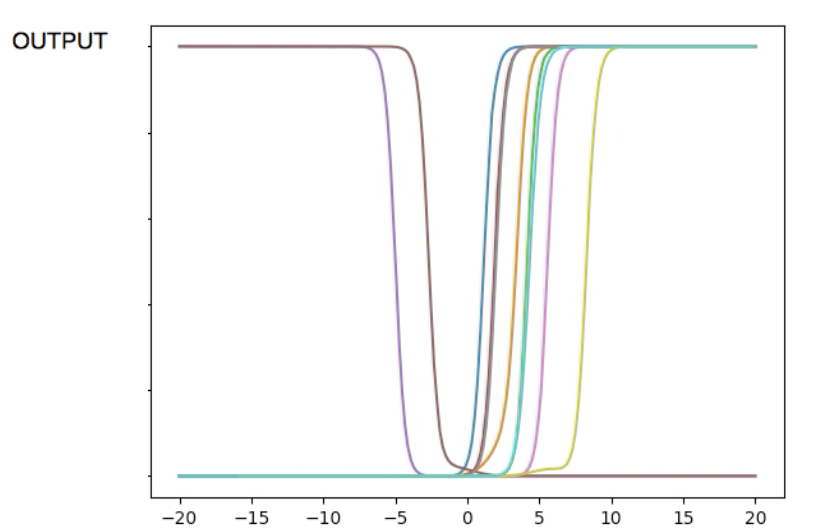
\includegraphics[width=5cm]{asset/output.png}


%%% Local Variables:
%%% mode: japanese-latex
%%% TeX-master: "./thesis"
%%% End:

\chapter{結論}
\label{conclusion}

本章では,本研究のまとめと今後の課題を示す.

\section{本研究のまとめ}

\section{本研究の課題}

%%% Local Variables:
%%% mode: japanese-latex
%%% TeX-master: "../thesis"
%%% End:

%\appendix
\chapter{ガウス分布とカーネル密度推定}


\section{K-AFの導出}
\label{appendix:calc}

本研究で実際に使用したアルゴリズムに用いた数式実際に導出する。
Ichimura(1993)~\cite{ichimura}の手法を用いてまずは以下の式に変換する。


\begin{eqnarray}
G(\mathbf{X}_iw)=\frac{\sum_{i\neq j} K\left(\frac{\mathbf{X}_j w - \mathbf{X}_i w}{h}\right)Y_j}{\sum_{i\neq j} K\left(\frac{\mathbf{X}_j w - \mathbf{X}_i w}{h}\right)}
\label{calc:k-af}
\end{eqnarray}

ここで、$ \sum_{i\neq j} K\left(\frac{\mathbf{X}_j w - \mathbf{X}_i w}{h}\right) \approx	\sum_{i\neq j} K\left(\frac{\mathbf{X}^{calc}_j w - \mathbf{X}_i w}{h_{calc}}\right)$
となるようなバンド幅$ h_{calc} $を見つけることで、全てのデータ点を使わなくとも$ \mathbf{X}_{calc} $を用いて\ref{calc:k-af}を近似することができる。

これにより\ref{calc:k-af}は以下の式に直すことができる。

\begin{eqnarray}
G(\mathbf{X}_iw) \approx \frac{\sum_{i\neq j} K\left(\frac{\mathbf{X}^{calc}_j w - \mathbf{X}_i w}{h_{calc}}\right)\mathbf{Y}^{calc}_j}{\sum_{i\neq j} K\left(\frac{\mathbf{X}^{calc}_j w - \mathbf{X}_i w}{h_{calc}}\right)}
\label{calc:k-af-2}
\end{eqnarray}

以上により、Ichimura(1993)raの手法に対してデータ点を減らしても近似できることを示した。


\chapter{カーネル活性化関数の実装}
\label{appendix:algorithm}


\section{クラス}


中間層が一つのK-AFの計算を考慮した実装クラスを\ref{python_impl}に示す。

実装の全ては \href{https://github.com/latte0/graduation\_thesis}{graduation\_thesis}. に公開している。

\begin{lstlisting}[caption=Pytorchを用いたK-AFの計算用のクラス,label=python_impl]
class Net(nn.Module):

    def __init__(self, Y, calc_Y, X, calc_X, settings):
        super(Net, self).__init__()

        self.fc1 = nn.Linear(DATA_INPUT_LENGTH, DATA_MID_LENGTH, bias=False)
        self.fc2 = nn.Linear(DATA_MID_LENGTH, DATA_OUTPUT_LENGTH, bias=False)
        # leave_ont_outのために事前に入力と出力をセットしておく
        self.Y = Y
        self.calc_Y = calc_Y
        self.calc = False
        # バンド幅も推定する
        self.h = nn.Parameter(torch.tensor(1.5, requires_grad=True))
        self.h_middle = torch.tensor(1.0)

        self.last_layer_result = []
        self.sigmoid = nn.Sigmoid()

    # kernel推定量の計算
    def kernel(self, Zw):
        numerator = 0
        denominator = 0
        result = []
        for j, \mathbf{X}_j in enumerate(self.train_X):

            Xw = self.fc2(F.relu(self.fc1(\mathbf{X}_j)))
            tmp = gauss((Xw - Zw) / self.h)

            tmp[j] = 0
            denominator += tmp
            numerator += tmp * self.Y[j]

        g = numerator/denominator
        return g


    def forward(self, x):

        xw = F.relu(self.fc1(x))
        xw = self.fc2(xw)

        y = self.kernel(xw)

        return y


\end{lstlisting}

また、活性化関数の学習が進んでいく様子を録画し、youtubeに公開している。



\begin{itemize}
  \item \href{https://github.com/latte0/graduation\_thesis}{実験1のwineの学習サンプル}
  \item \href{https://github.com/latte0/graduation\_thesis}{実験1のwineの学習サンプル}
  \item \href{https://github.com/latte0/graduation\_thesis}{実験1のwineの学習サンプル}
  \item \href{https://github.com/latte0/graduation\_thesis}{実験1のwineの学習サンプル}
  \item \href{https://github.com/latte0/graduation\_thesis}{実験1のwineの学習サンプル}
\end{itemize}


\chapter*{謝辞}
\addcontentsline{toc}{chapter}{謝辞}
\label{thanks}

本論文の執筆にあたり、ご指導頂いた慶應義塾大学環境情報学部教授村井純博士、同学部教
授中村修博士、同学部教授楠本博之博士、同学部准教授高汐一紀博士、同学部教授三次仁
博士、同学部准教授植原啓介博士、同学部准教授中澤仁博士、同学部準教授 Rodney D。
Van Meter III 博士、同学部教授武田圭史博士、同大学政策・メディア研究科特任准教授
鈴木茂哉博士、同大学政策・メディア研究科特任准教授佐藤 雅明博士、同大学 SFC 研究
所上席所員斉藤賢爾博士に感謝致します.

特に斉藤氏には重ねて感謝致します。研究活動を通して技術的視点、社会的視点等の
様々な視点から私の研究に対して助言を頂き、深い思考と学びを経験させて頂くことがで
きました。これらの経験は私の人生において人・学ぶ者として、素敵な財産として残りま
した。博士の指導なしには、卒業論文を執筆することは出来ませんでした。

徳田・村井・楠本・中村・高汐・バンミーター・植原・三次・中澤・武田合同研究プロ
ジェクトに所属している学部生、大学院生、卒業生の皆様に感謝致します。研究会に所属
する多くの方々が各々の分野・研究で奮闘している姿を見て学んだことが私の研究生活を
より充実したものとさせました。

異なる分野同士が触れ合い、学び合う環境に出会えたことを嬉しく感じます。
また、NECO 研究グループとして多くの意見・発想・知見を与えてくださった、慶應義
塾大学政策メディア・研究科 阿部涼介氏、卒業生 菅藤佑太氏、在校生 島津翔太氏、
宮本眺氏、渡辺聡紀氏、梶原留衣氏、渡辺聡紀氏、木内啓介氏、後藤悠太氏、倉重健氏、
九鬼嘉隆氏、相原航平氏、小島大季氏、吉開拓人氏、金城奈菜海氏、長田琉羽里氏、
崔仁珠氏、上倉隼氏、田崎和輝氏に感謝致します。

村井純研究室統計的機械学習グループの小林凌雅氏、政策メディア研究科博士後期課程 川本章大氏、同研究科修士課程 幅野莞佑氏、
環境情報学部学士課程 岩崎智也氏、株式会 社 SIMULA Labs CEO 牧野暉弘氏、EMC Healthcare 株式会 社 深澤風土氏、
一橋大学経済 学研究科 田柳敏和氏に感謝します。
SL で共に研究について議論をし、学ぶことができた 経験は一生の財産になりました。重ねて感謝申し上げます。

特に研究について幾度となく議論に付き合ってくださった小林凌雅氏には重ねて感謝します。
研究のアイディアの段階から様々な指摘やアドバイスをしていただきました。
小林凌雅氏の存在なしにはこの論文は存在しなかったと思います。
研究の他にもここでは書ききれないほど多くのことで支えていただきました。
最後にもう一度重ねて感謝申し上げます。

皆様には、私の研究に対する多くの助言や発想を頂いただけでなく、研究活動における
学びを経験させて頂きました。
多くの出会いと学びの環境である SFC に感謝致します。多様な学問領域に触れ、学生
同士で議論し思考することが出来ました。幸せで素敵な時間でした。

最後に、これまで私を育て、見守り、多くの学びの機会並びに本卒業論文執筆の機会を
与えてくれた、両親と兄に感謝致します



%%% Local Variables:
%%% mode: japanese-latex
%%% TeX-master: "../yummy_bthesis"
%%% End:


\renewcommand{\thechapter}{\Alph{chapter}}
\setcounter{chapter}{0}
\vspace{-5mm}


\bibliographystyle{unsrt}\pagestyle{plain}
\bibliography{./bib/cites}\pagestyle{plain}
\thispagestyle{plain}%bibtex


\end{document}

%%% Local Variables:
%%% mode: japanese-latex
%%% TeX-master: t
%%% End:
